%\section{Results}
%\label{sec:Results}
%% Results should be clear and concise.

The experiment to test the hypothesis that participants in a virtual reality (VR) experiment would show a trend towards choosing complex environments over simple ones when given the task of identifying the more comfortable facade design, was conducted at the Kyushu University campus in Fukuoka, Japan, over a period of 15 days, from October 12 to 30, 2023, during the work hours between 10:00 and 18:00.

A total of \(10\) participants took part in the experiment, primarily consisting of university students and faculty members.
The participants had diverse professional backgrounds, as shown in Figure \ref{fig:SurveyBackgroundChart}, with over \(67\%\) being students from various faculties, approximately \(33\%\) having a construction background, and \(14\%\) reporting previous experience in facade design, as indicated in Figure \ref{fig:SurveyYearsExperienceChart}

%% Participant background chart and years of experience
    \begin{table*}[htb]
        \centering
        \small
        \begin{tabularx}{\textwidth}{X X}
            \centering
            % trim=left 0 down 50 right 0 top 50
            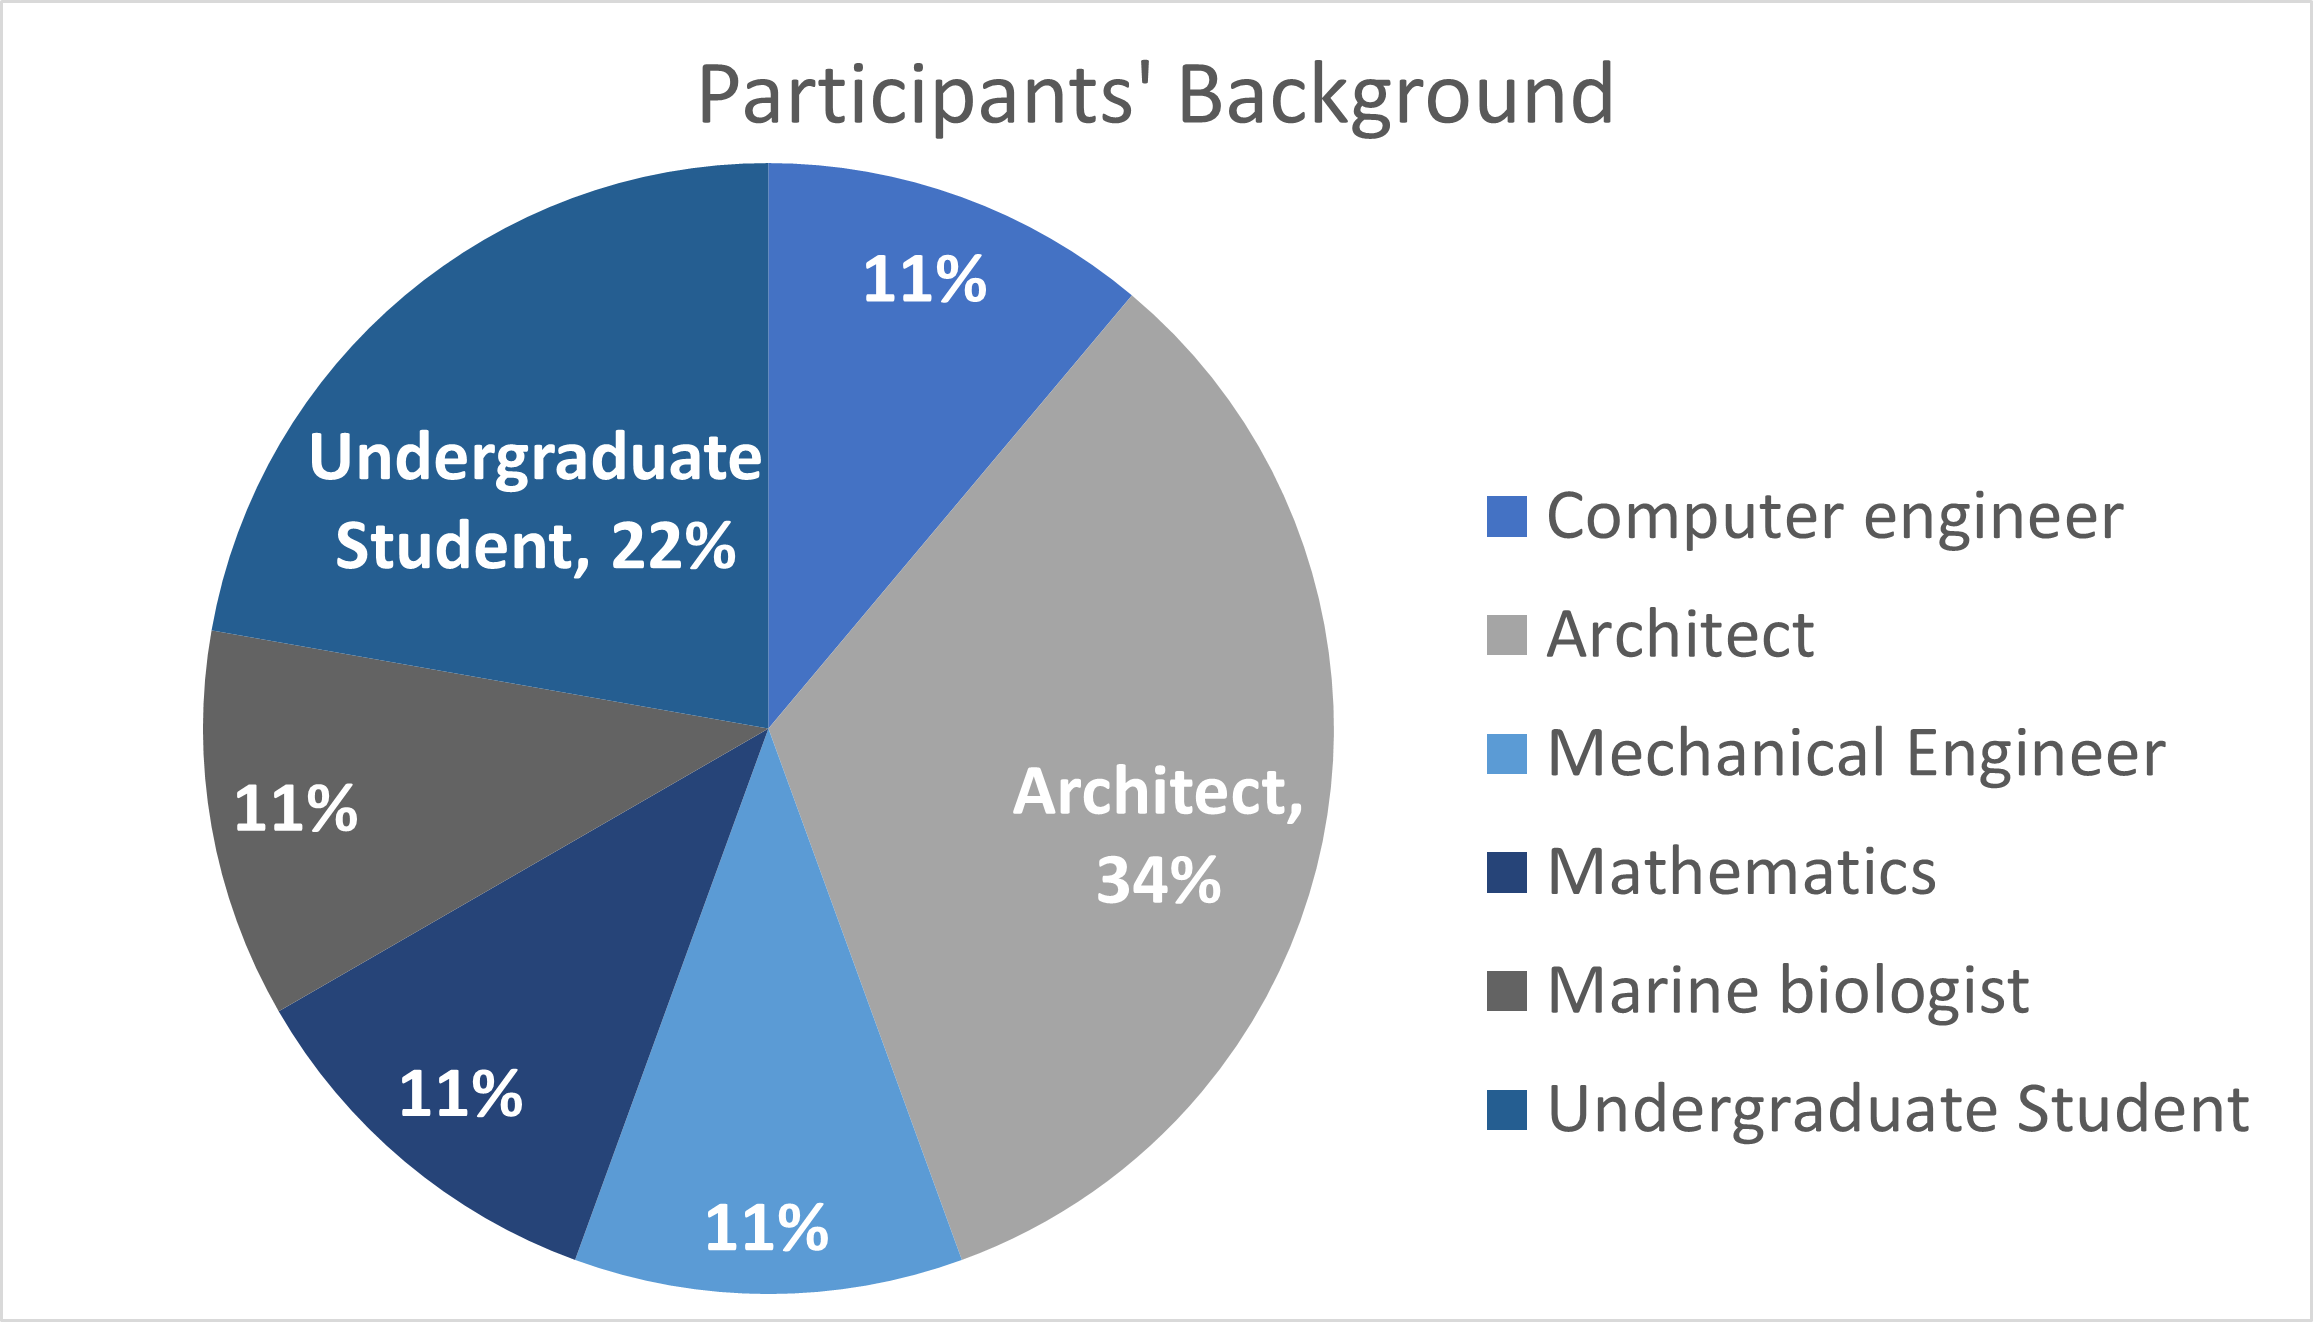
\includegraphics[width=\linewidth, trim=0 60 0 0]{Images/SurveyBackground}
            \captionof{figure}{This chart shows the professional backgrounds of participants involved in the facade design complexity analysis experiment.}
            \label{fig:SurveyBackgroundChart} &
            \centering
            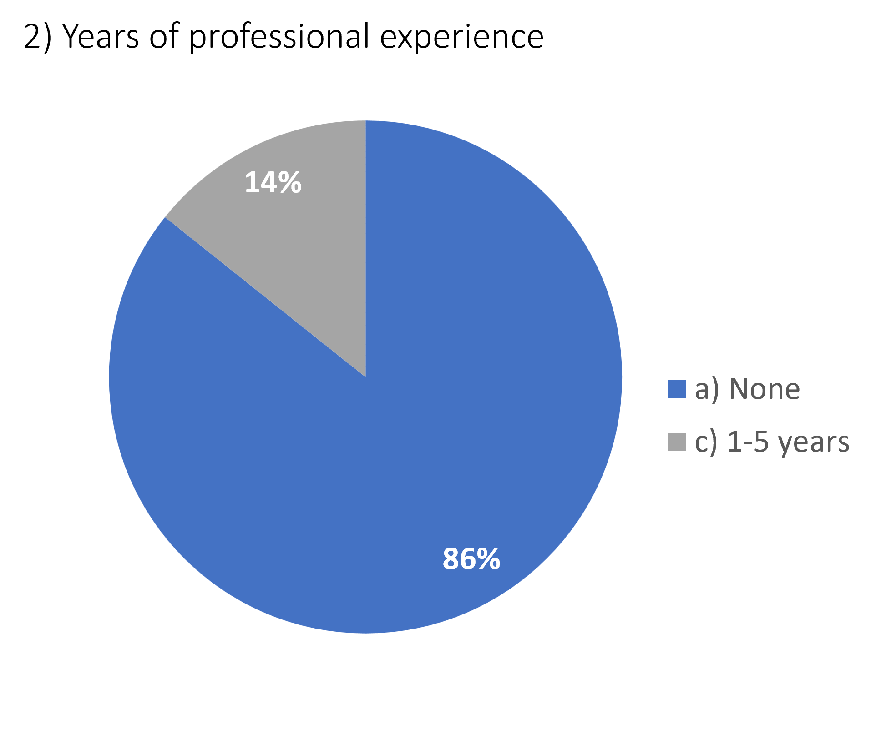
\includegraphics[width=\linewidth, trim=0 60 0 0]{Images/SurveyExperience}
            \captionof{figure}{This chart displays the experience levels in facade design of participants for the study complexity analysis in building design.}
            \label{fig:SurveyYearsExperienceChart}
        \end{tabularx}
    \end{table*}

In the `VR Interaction' stage, which focused on assessing user tolerance for complex facade designs, each participant completed the facade selection task for all three patterns, resulting in a total of 30 experiment sessions.
For each pattern, participants provided one answer, indicating their preference for the facade variation labeled with a complexity level that they found the most comfortable.

%!Complexity level chosen bar chart
These outcomes were summarized in a bar chart referred to as `Complexity level Chosen graph' as depicted in Figure \ref{fig:ComplexityLevelChosenChart}.

    % Complexity level chosen Chart
    \begin{figure}[htb]
        \centering
        %trim=100 180 100 120, clip
        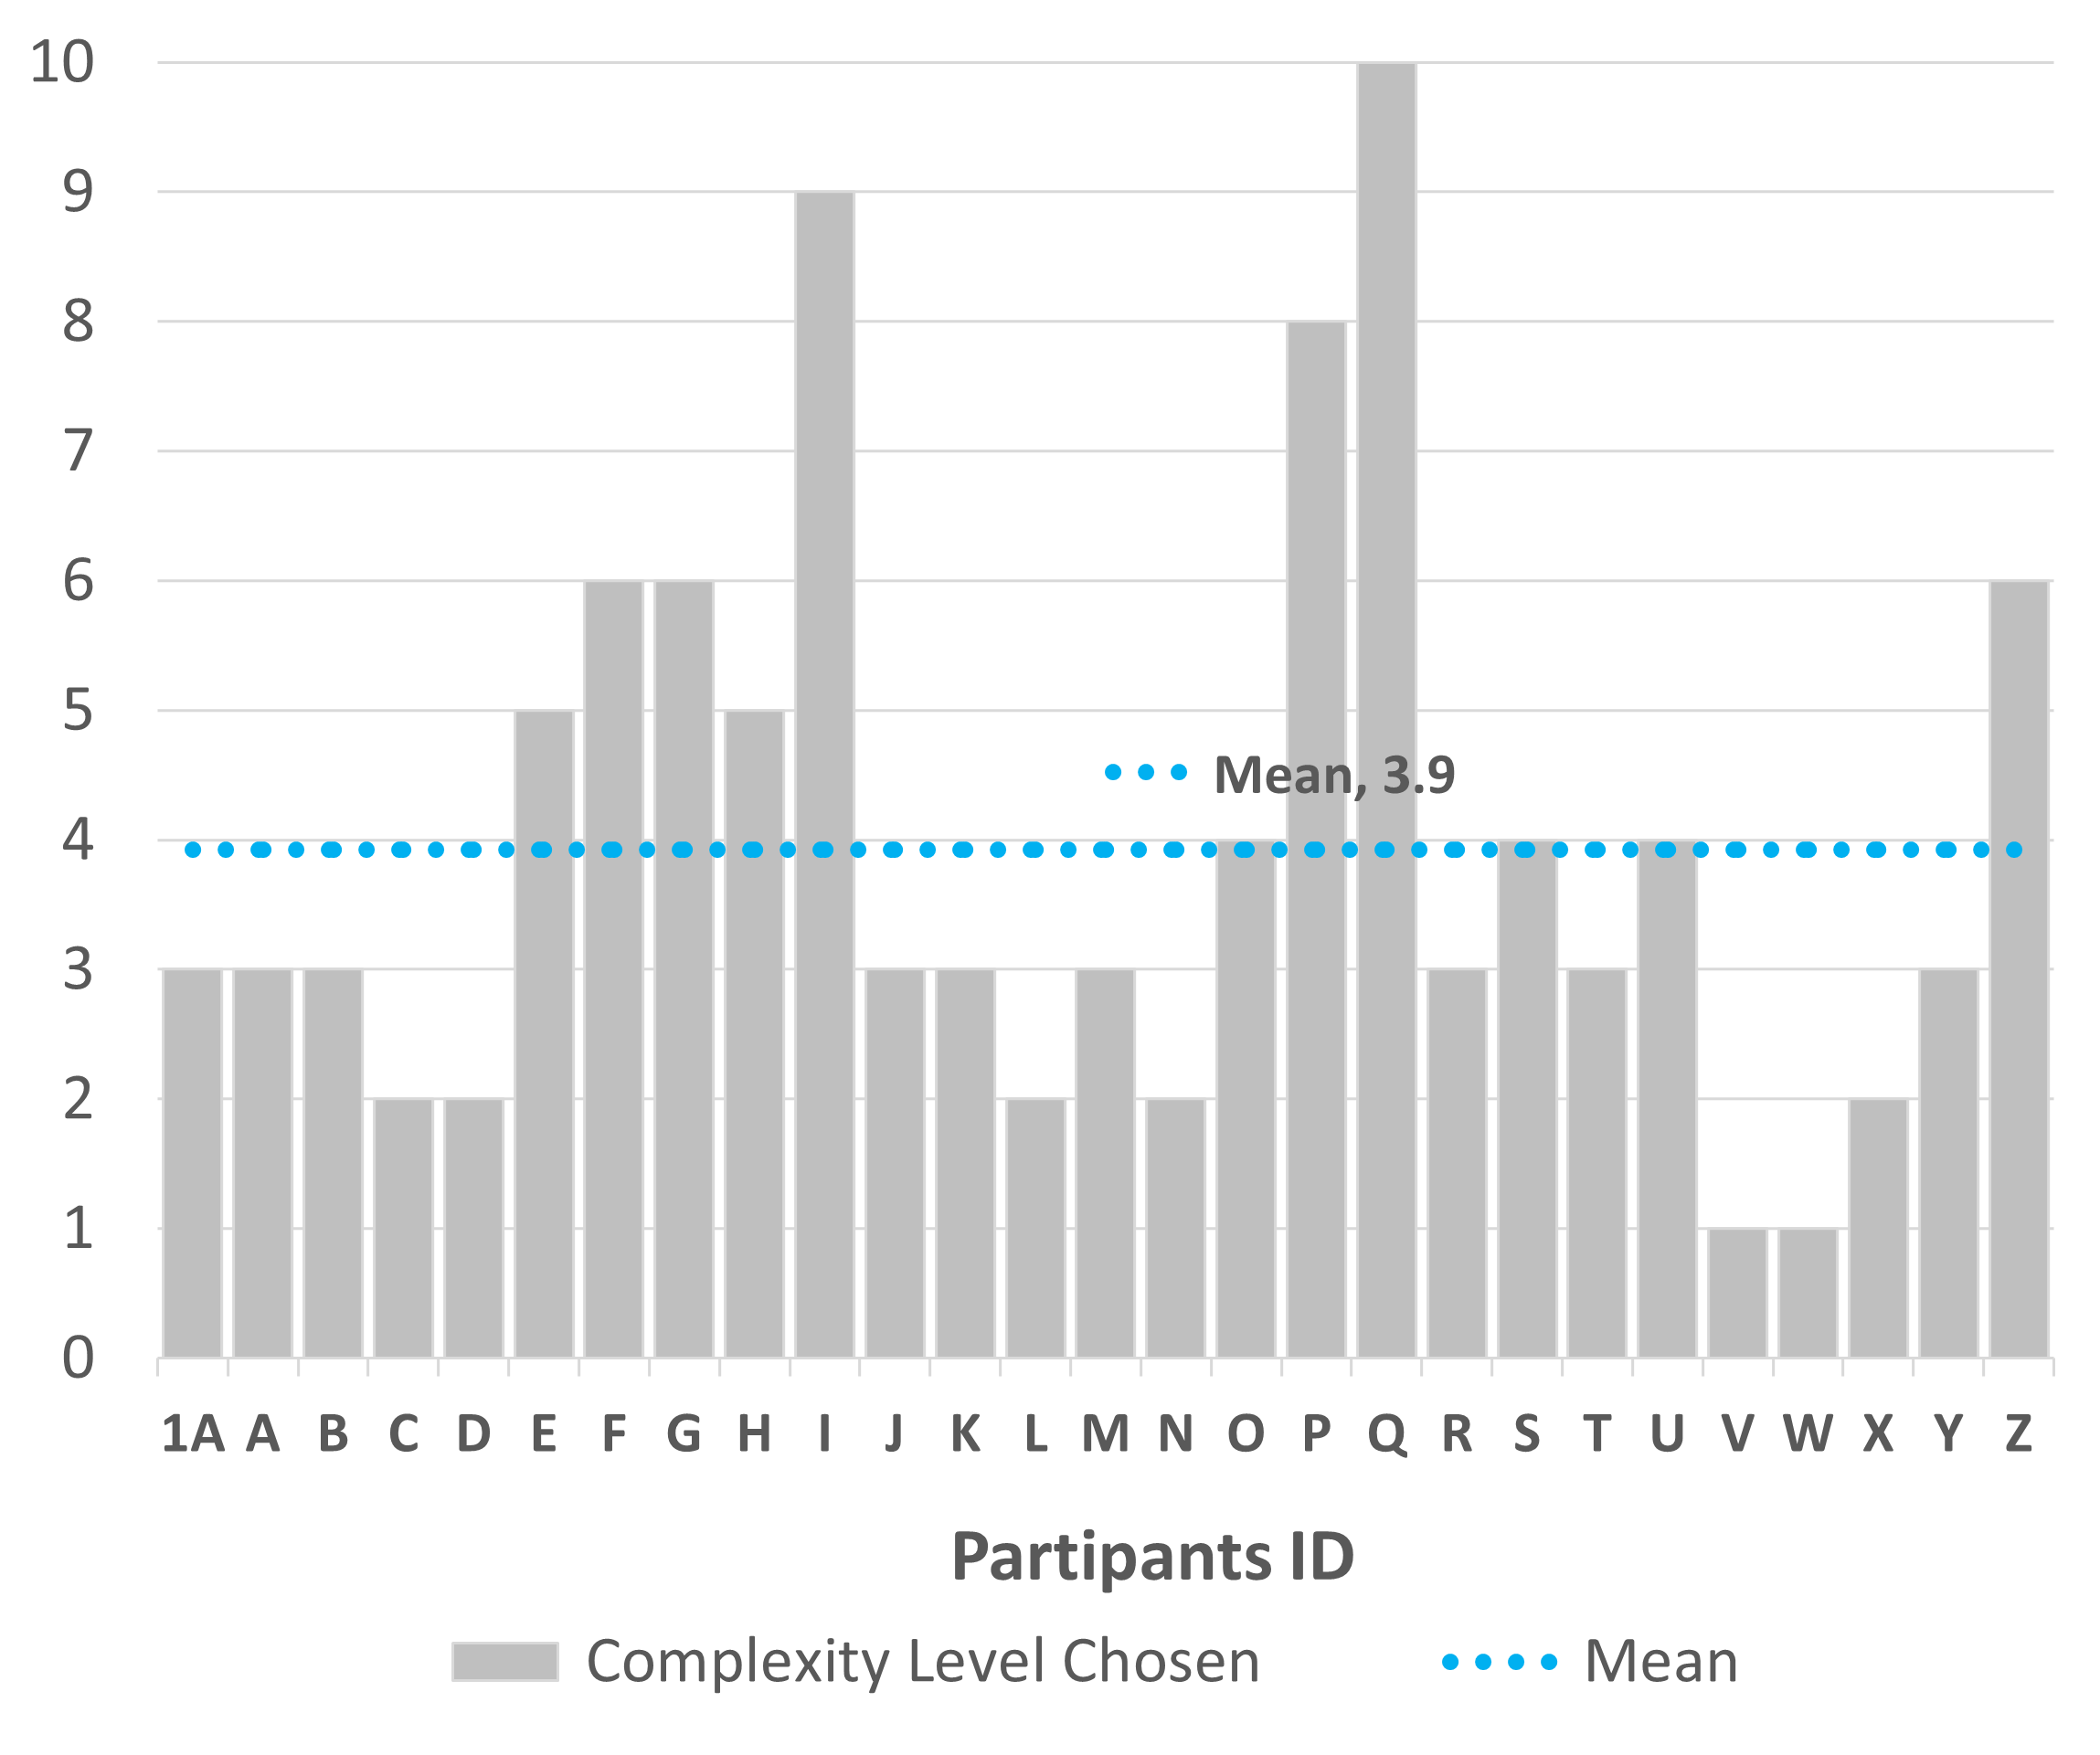
\includegraphics[width=\linewidth]{Images/ComplexityLevelChosenChart}
        \caption{Chart displaying participants' preferred complexity levels among the ten options during the VR simulation stage of the experiment for all three patterns.}
        \label{fig:ComplexityLevelChosenChart}
    \end{figure}

The Complexity chosen level results, depicted in the `Complexity level Chosen graph' in Figure \ref{fig:ComplexityLevelChosenChart}, showcased a diverse range of preferences among the 30 experiment sessions, with most of them allocated bellow the `level 5' of complexity and only five instances going above this line, returning overall an average of  complexity level \(3.9\) as the preferred one among the 10 levels defined for the facade variations for all three patterns.

The preferred complexity level depicted on this graph exhibited a wide distribution, as indicated by the current standard deviation of \(2.3\).

%!Complexity level chosen probability graph

The probability bell graph displayed in Figure \ref{fig:ProbabilityComplexitylevelChart} further illustrates the distribution of choices in the results, emphasizing that there is a \(40\%\) probability of a focus group selecting and answer close to the level 4 of complexity as defined by the facade variations with a standard deviation of \(11\%\)in predicting individual data points or outcomes.

     % Probability Chart and Complexity level per Pattern
    \begin{table*}[htb]
        \centering
        \small
        \begin{tabularx}{\textwidth}{X X}
            \centering
            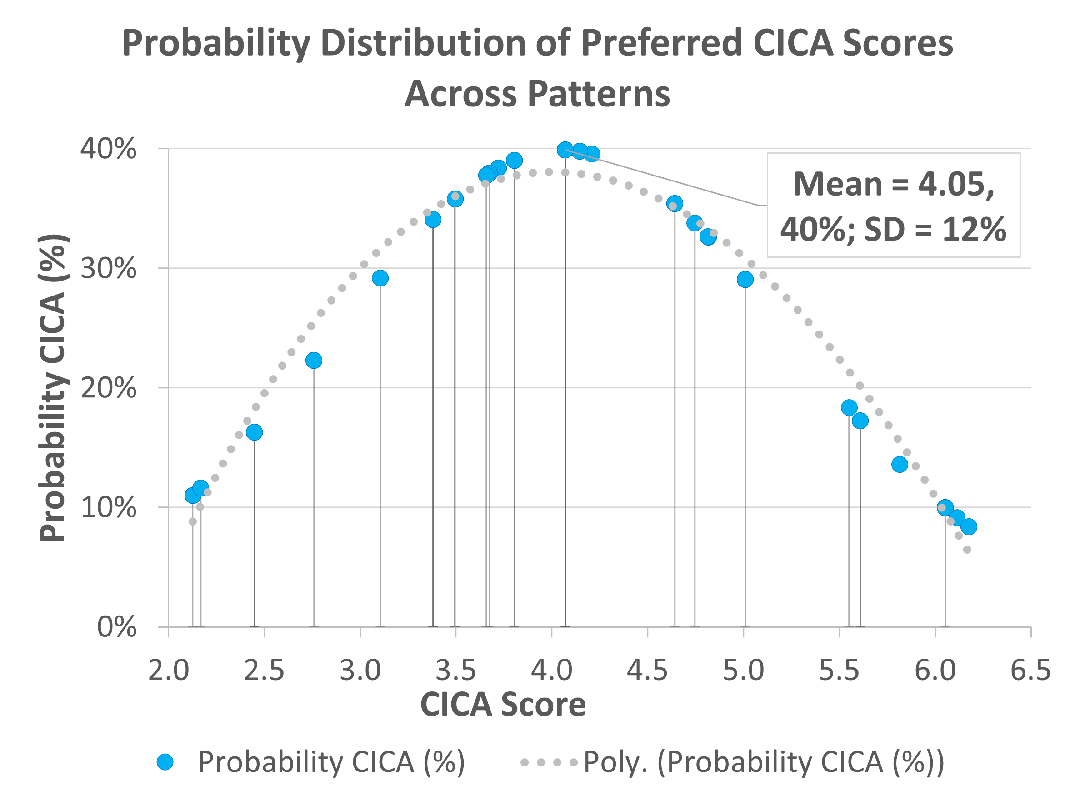
\includegraphics[width=\linewidth, trim=0 0 0 20]{Images/ProbabilityPreferredComplexitylevel}
            \captionof{figure}{Scatter graph illustrating the probability distribution of preferred complexity levels for facade design across all three patterns, derived from data collected during the VR stage of the experiment.}
            \label{fig:ProbabilityComplexitylevelChart} &
            \centering
            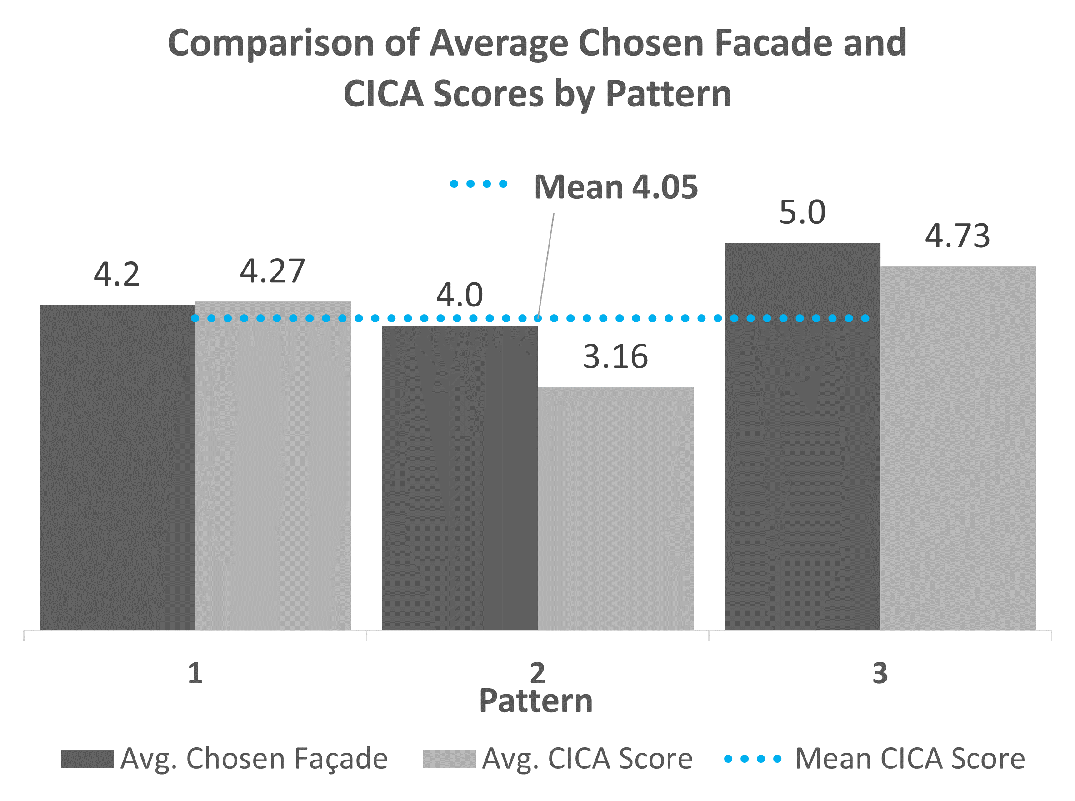
\includegraphics[width=\linewidth, trim=0 0 0 20]{Images/PreferredComplexityLevelPerPattern}
            \captionof{figure}{Average preferred complexity level per pattern by participants during the VR simulation (Overall Mean complexity level = \(4.9\)).}
            \label{fig:ComplexityLevelPerPattern}
        \end{tabularx}
    \end{table*}

%% probability preferred complexity level Chart
%    \begin{figure}[htb]
%        \centering
%        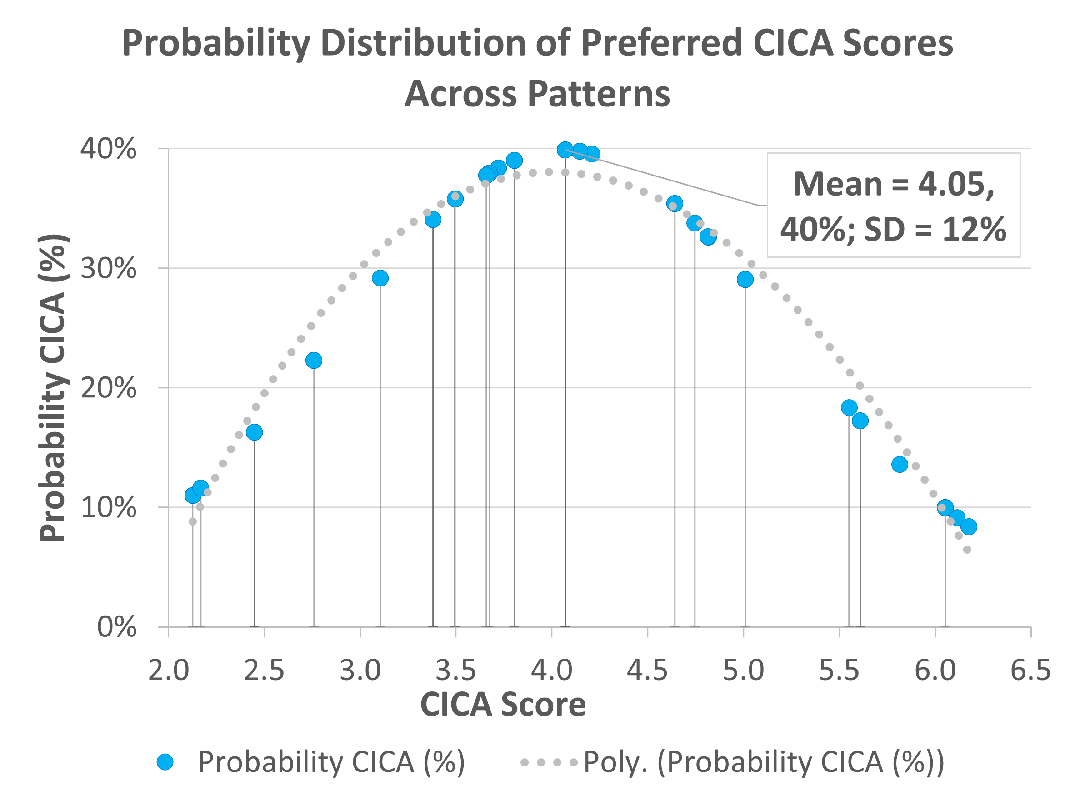
\includegraphics[width=\linewidth]{Images/ProbabilityPreferredComplexitylevel}
%        \caption{Scatter graph illustrating the probability distribution of preferred complexity levels for facade design across all three patterns, derived from data collected during the VR stage of the experiment.}
%        \label{fig:ProbabilityComplexitylevelChart}
%    \end{figure}

%!Complexity level per pattern graph

Analyzing the average complexity level chosen per pattern by the experiment participants, summarized in the graph in Figure \ref{fig:ComplexityLevelPerPattern}, it is once again revealed that the average choice across all patterns remains close to the overall average complexity level \(3.9\), with \(3.9\) for pattern 1, \(4.2\) for pattern 2, and \(3.9\) for pattern 3.

%===============Continue from here for the accuracy section

%!Complexity perception per level with trendlines

In terms of the accuracy of the ‘Computational Image Complexity Analysis’ (CICA) system in evaluating the complexity of facade variations in comparison to the perceptions of the participants, the results are illustrated in the Column chart in Figure \ref{fig:ComplexityPerceptionPerLevel}, where the trendlines for all three patterns show a similar trajectory to the trendline obtained from the original ranking with an average standard deviation of \(1\) in complexity level categorisation.

 %% Figure Complexity perception per level with trendlines
    \begin{figure*}[htb]
      \centering
      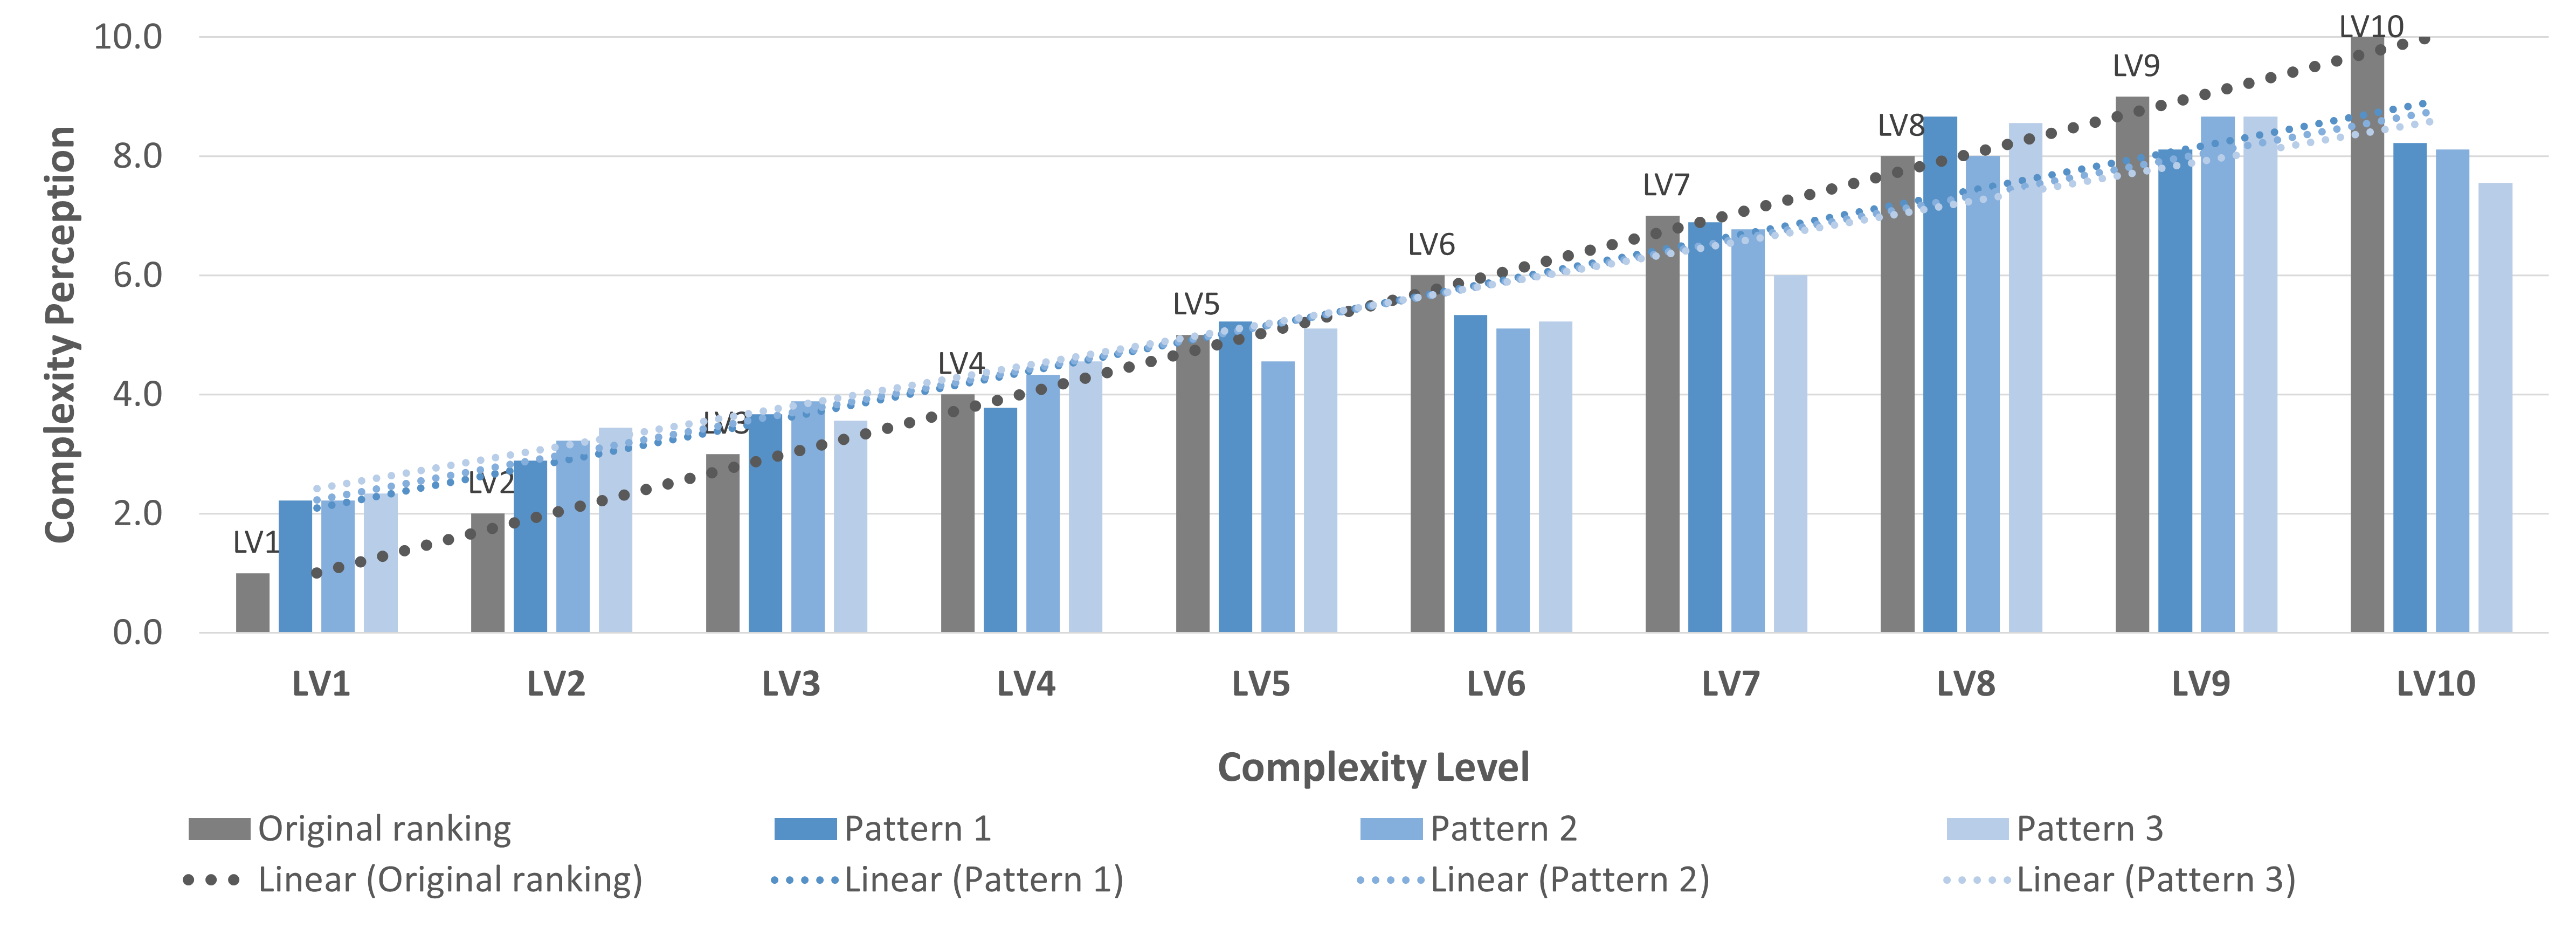
\includegraphics[width= \linewidth, trim=0 0 0 0]{Images/ComplexityPerceptionPerLevel}
      \caption{This graph highlights participants' perception of complexity for the 10 variations within three patterns in contrast to the original ranking. It visually represents the differences between participants' perceived complexity and the initial rankings during the screen-based complexity assessment stage of the experiment.}
      \label{fig:ComplexityPerceptionPerLevel}
    \end{figure*}

%!Complexity perception per pattern

The comparison between the perception of the participants and the original ranking illustrated per pattern and displayed in Figure \ref{fig:ComplexityPerceptionChart}, shows how the results from the experiment create a close to similar shape to the one organized by the original ranking following a similar trajectory.


% Figure Complexity perception Chart per pattern
    \begin{figure}[htb]
        \centering
        %trim=100 180 100 120, clip
        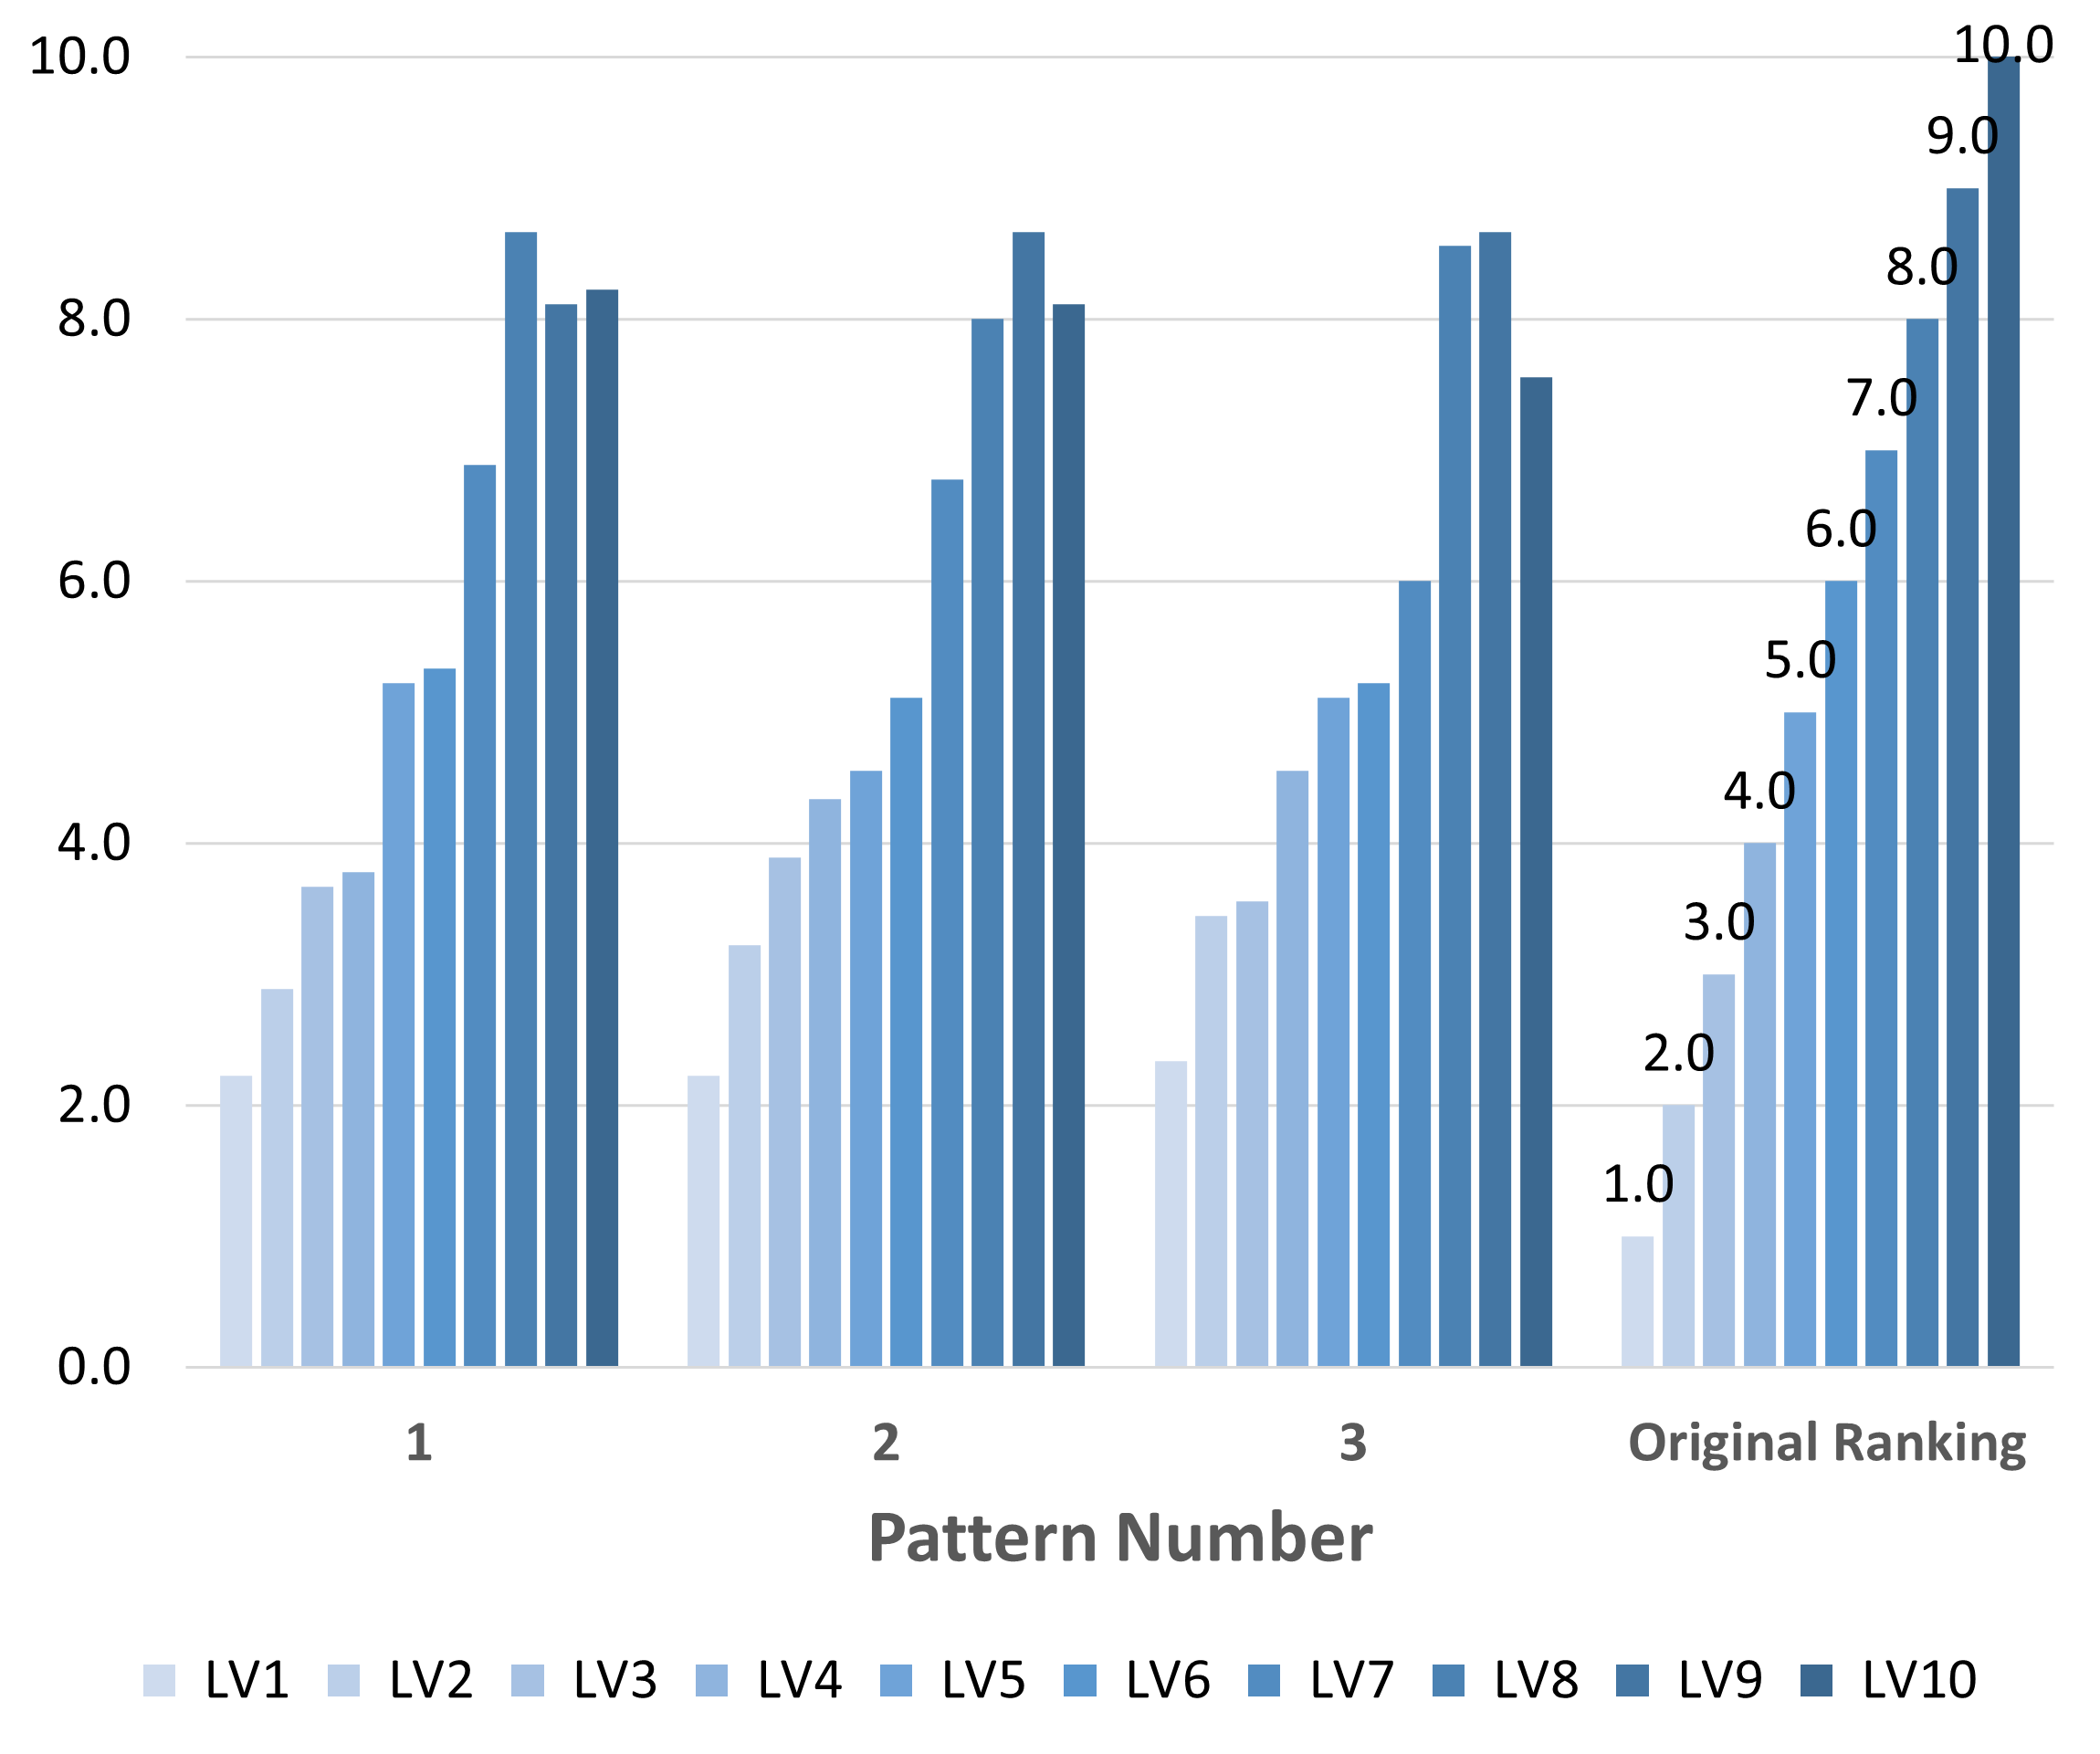
\includegraphics[width=\linewidth]{Images/ComplexityPerceptionChart}
        \caption{Chart depicting participants' complexity perception related to the three patterns. Insights into participants' perception of complexity concerning specific patterns during the screen-based complexity assessment phase of the experiment.}
        \label{fig:ComplexityPerceptionChart}
    \end{figure}

The purpose of the analysis was to evaluate the deviation error between the original ranking given by the CICA system and the one ultimately established by the experiment participants given during the `screen-based ranking' stage of the experiment.

By determining the deviation error, this analysis allowed us to quantify the accuracy of the CICA system in predicting complexity levels in facade design.

The accuracy analysis results, depicted in Figure \ref{fig:ComplexityPerceptionPerLevel} and in Figure \ref{fig:ComplexityPerceptionChart}, showcased varying degrees of accuracy between facade variations and across patterns with an average deviation of \(0.9\) for pattern 1, \(0.9\) for pattern 2, and \(1.1\) for pattern 3, with the largest deviation errors allocated at both the lowest and highest level of complexity.

%! Post experiment survey results

The survey results offer valuable insights into how building users perceive facade complexity and the factors influencing their facade design preferences.
The responses to the 'complexity perception' section of the survey have been summarized in Figures \ref{fig:SurveyQuestions6-10} and \ref{fig:SurveyQuestions11-15}, with evaluations conducted using a 7-point Likert scale.

  %% Complexity Perception Survey results
    \begin{table*}[htb]
        \centering
        \small
        \begin{tabularx}{\textwidth}{X X}
            \centering
            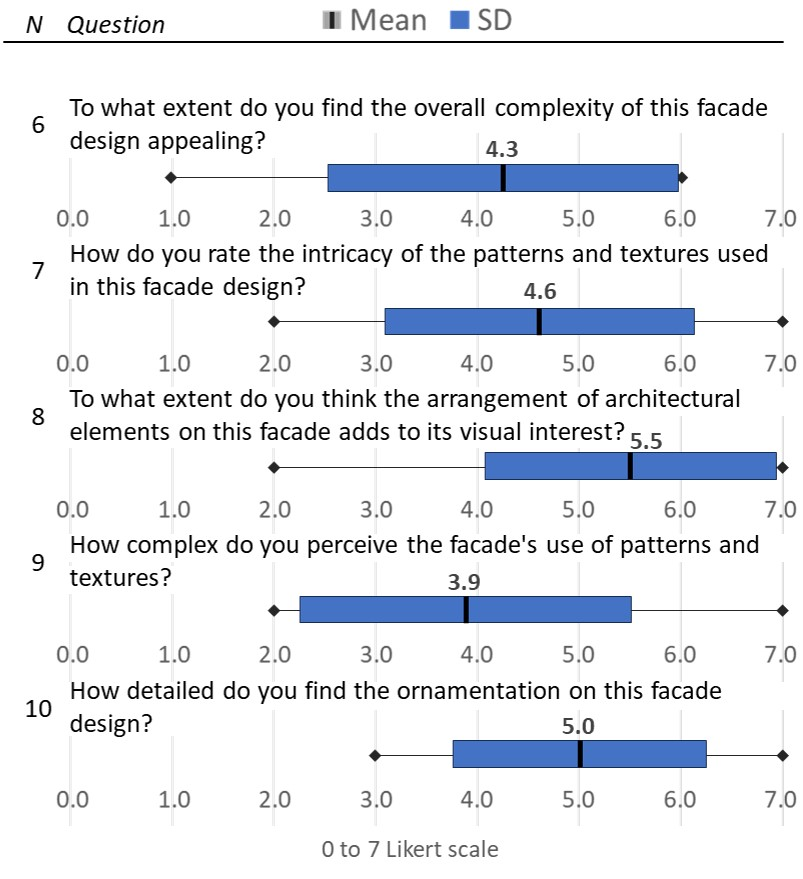
\includegraphics[width=\linewidth]{Images/SurveyPart1Complexity}
            \captionof{figure}{Questions 6 to 10 of the Complexity perception section from the Post-Experiment Survey. \- (n = 10), 1 - strongly disagree, 7 - strongly agree}
            \label{fig:SurveyQuestions6-10} &
            \centering
            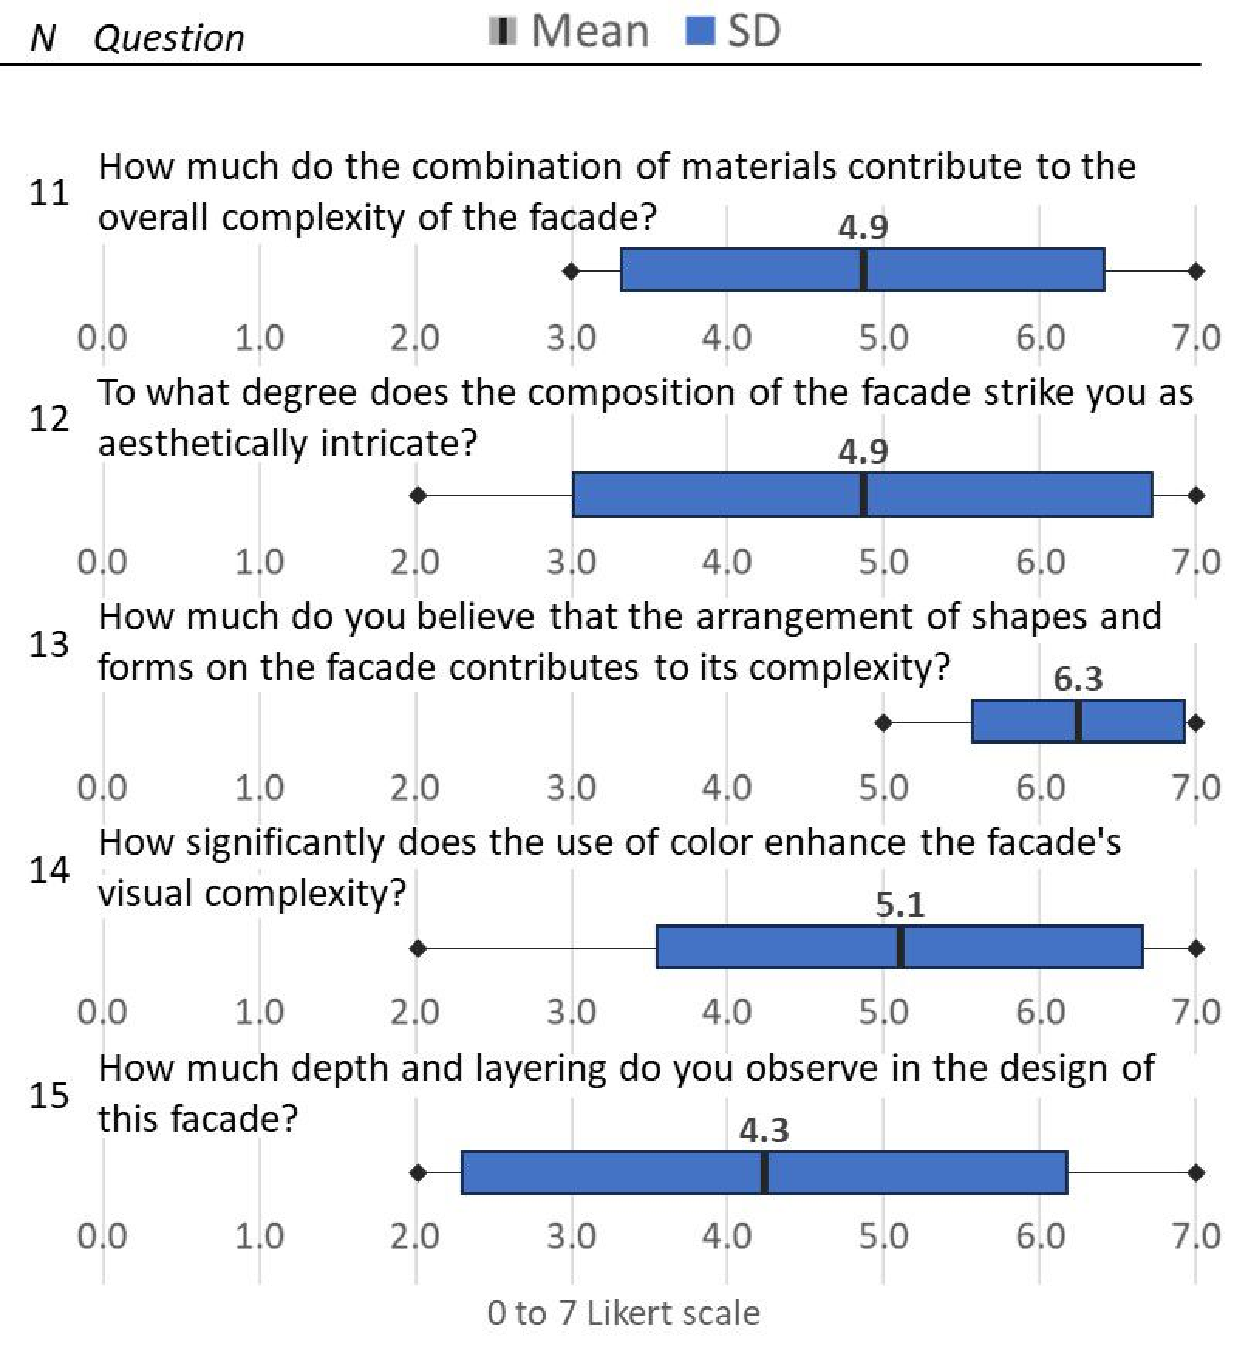
\includegraphics[width=\linewidth]{Images/SurveyPart2Complexity}
            \captionof{figure}{Questions 6 to 10 of the Complexity perception section from the Post-Experiment Survey. \- (n = 10), 1 - strongly disagree, 7 - strongly agree}
            \label{fig:SurveyQuestions11-15}
        \end{tabularx}
    \end{table*}

Notably, all the questions garnered scores exceeding \(3.5\), with an average rating of \(4.9\).
This indicates a generally favorable attitude among respondents toward classifying the presented facade variations as complex.
However, the average standard deviation of \(1.5\) reveals a degree of variability in responses.

In other words, the responses are somewhat scattered around the mean (average).
This dispersion suggests that while some participants provided highly positive ratings (above the mean), others offered less enthusiastic assessments (below the mean).
These variations in responses underscore the diverse perspectives and preferences among participants, enriching our understanding of how users perceive facade complexity.


%! Detailed analysis of survey questions
Further analysis suggests .....................

Regarding the aesthetical appeal of the prepared facade variation design the overall consensus

%! Post experiment interview

During post-experiment interviews, participants were asked to express their views on the relative importance of form and materials when evaluating facade.
Remarkably, the responses were unanimous, with participants consistently favoring form over materials as the more significant criterion.
Additionally, participants indicated a clear preference for a weight distribution of \(80\%\) for form and \(20\%\) for materials in their decision-making process when assessing facade complexity.

Regarding intricate facade designs, another consensus among participants was the emphasis on views.
Given the experiment's location, which affords a front view of the entire campus and a side view facing another building, participants expressed a clear preference for an unobstructed facade on the front view.
They suggested that a facade design capable of framing and enhancing the campus view would be preferable over an intricate pattern.

Conversely, for the side of the building facing the neighboring structure, participants favored intricate patterns that offered increased privacy or complexity.
In this context, the view of the neighboring building was considered less important to preserve, and participants believed that a complex facade could enhance both the building's aesthetic appeal and privacy.

%! Preliminary Conclusion

In summary, the findings align with our initial hypothesis, indicating a trend in contemporary architecture towards increasingly complex facade designs.
This shift is evident not only in the quantitative analysis of historical facade complexity trends, as illustrated in Figure \ref{fig:complexitygraph}, but also in the results of our experimental phase.

Participants in the experiment displayed a clear inclination towards complexity, with an average complexity level selection of \(3.9\).
This suggests ample room for the incorporation of complex forms in contemporary building and facade design.
This observation is further reinforced by the overall positive reception of the facade variations in the post-experiment survey, with an average rating of \(4.9\) on a 7-point Likert scale.
Participants consistently characterized the presented facades as both aesthetic and intricate.

Taken together, these findings support the notion that contemporary architecture is embracing complexity in facade design, marking a departure from more simplistic interpretations of architecture associated with the guidelines of modernist movement.


%! preview accuracy graphs alternative
\ref{fig:AccuracyPattern1}\ref{fig:AccuracyPattern2}\ref{fig:AccuracyPattern3}
  %% Complexity Perception Survey results
    \begin{table*}[htb]
        \centering
        \small
        \begin{tabularx}{\textwidth}{X X X}
            \centering
            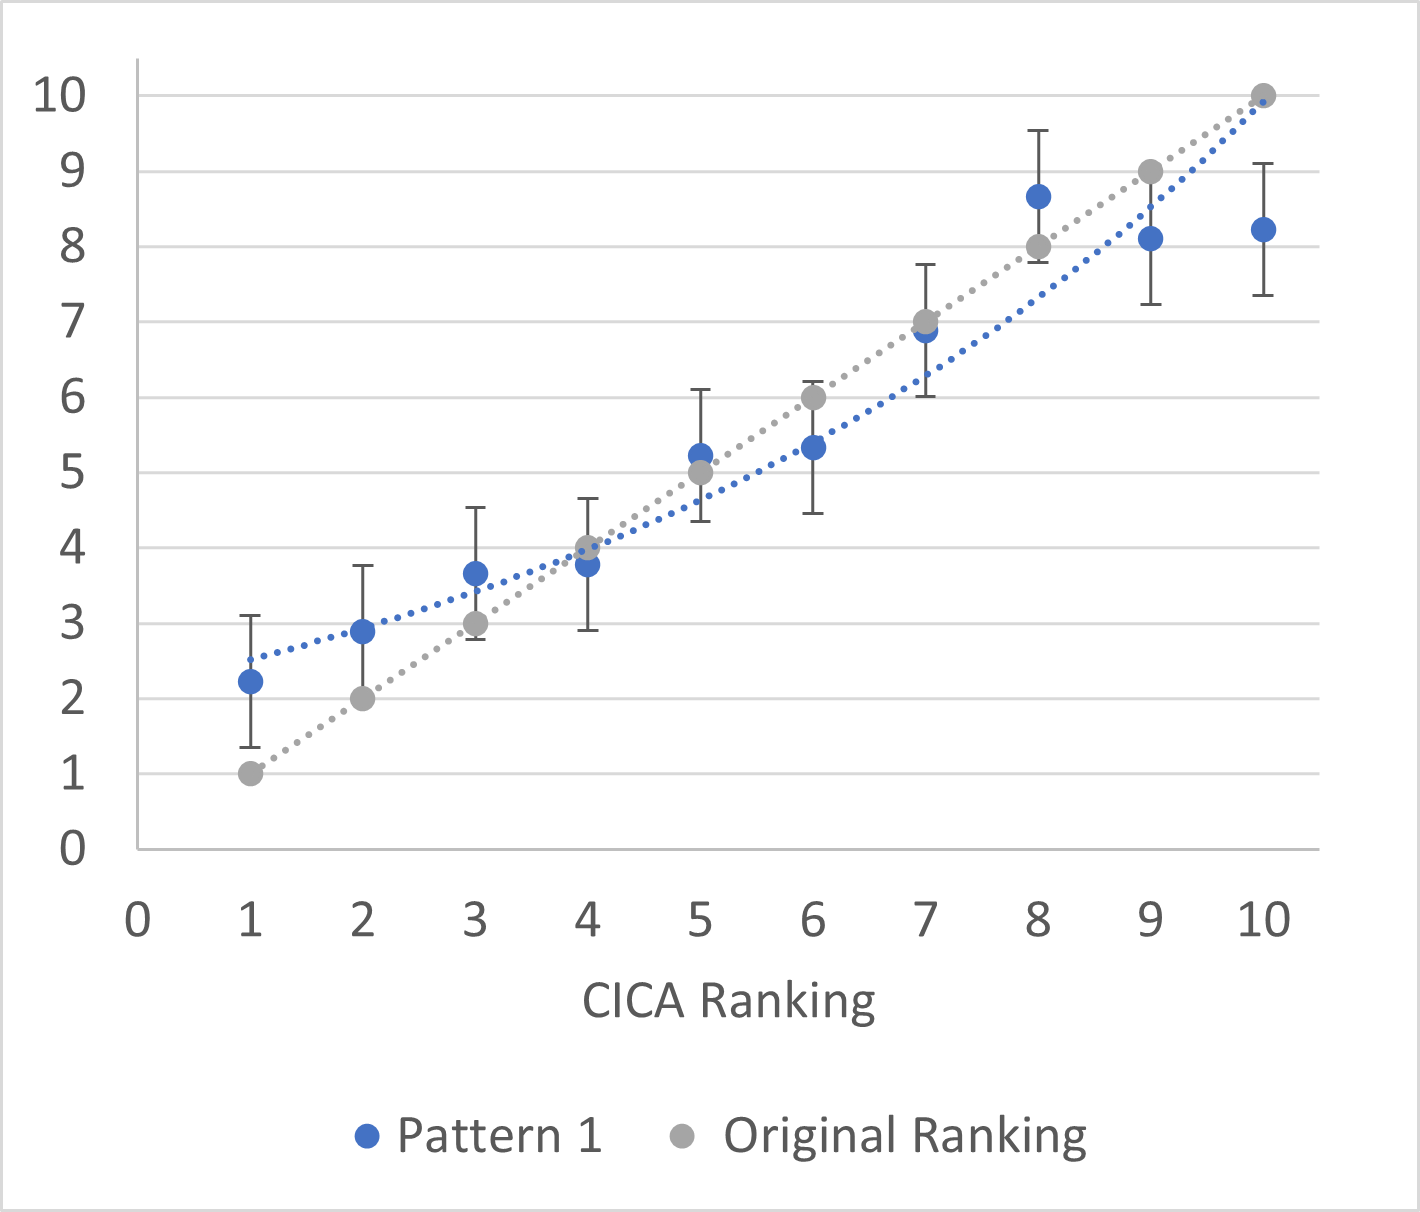
\includegraphics[width=\linewidth]{Images/AccuracyPattern1}
            \captionof{figure}{Accuracy comparison pattern 1 with original ranking}
            \label{fig:AccuracyPattern1} &
            \centering
            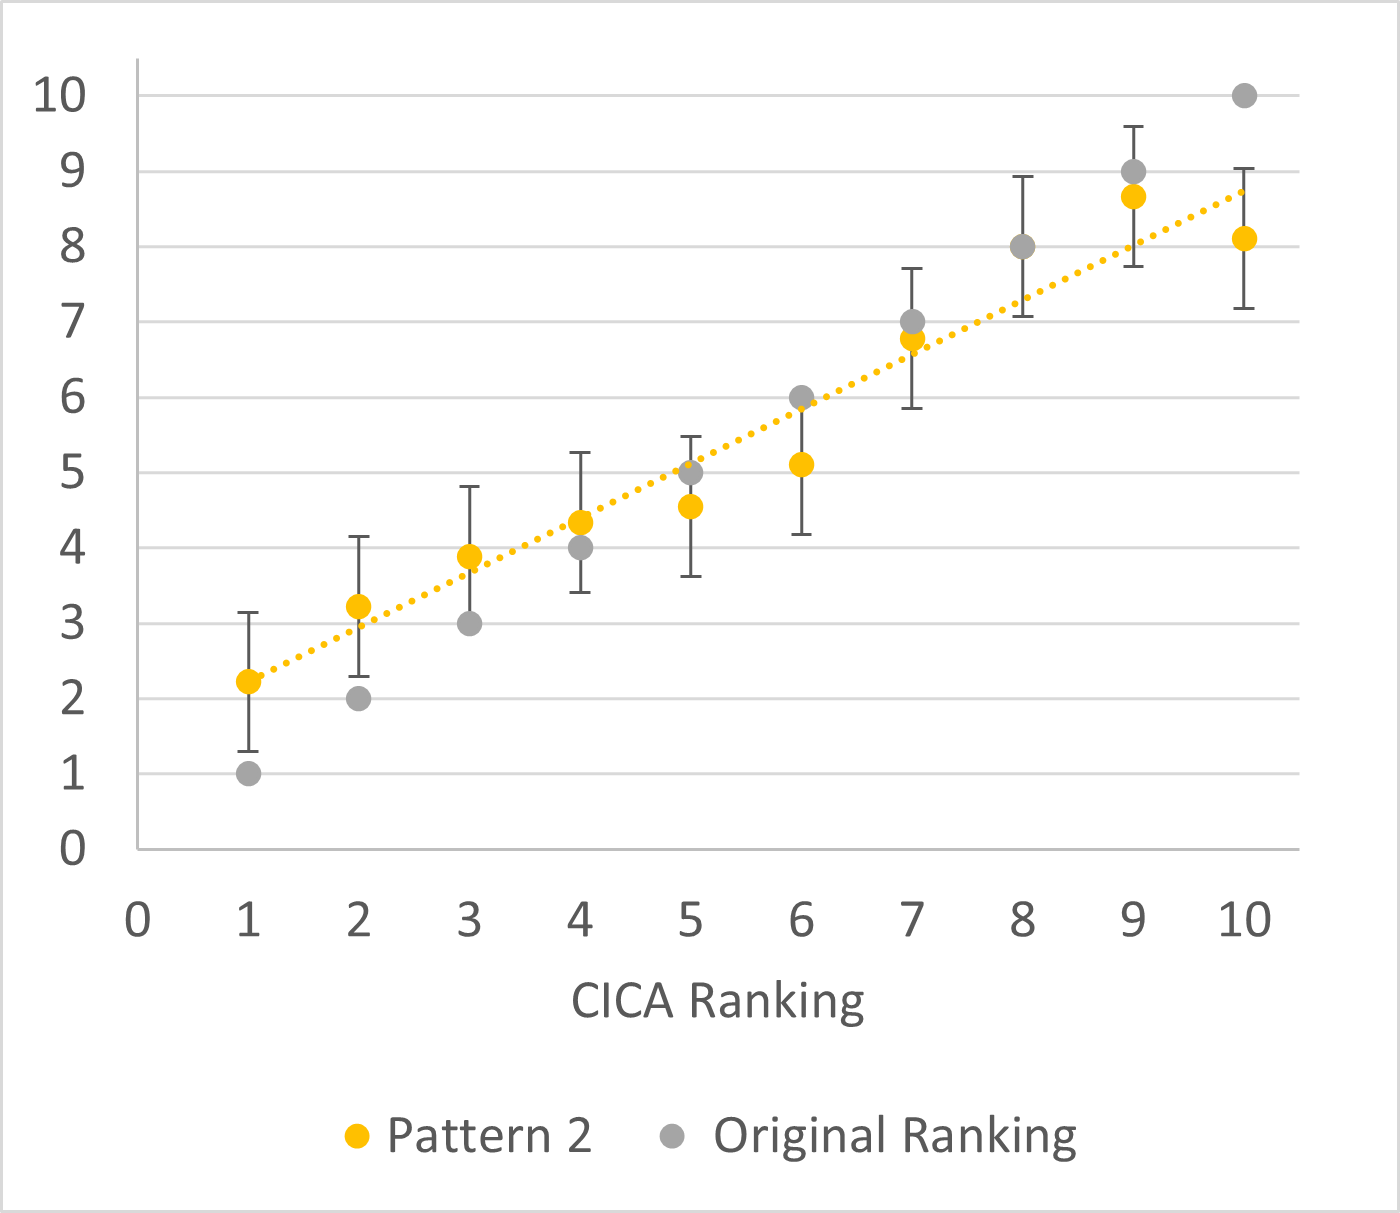
\includegraphics[width=\linewidth]{Images/AccuracyPattern2}
            \captionof{figure}{Accuracy comparison pattern 2 with original ranking}
            \label{fig:AccuracyPattern2} &
            \centering
            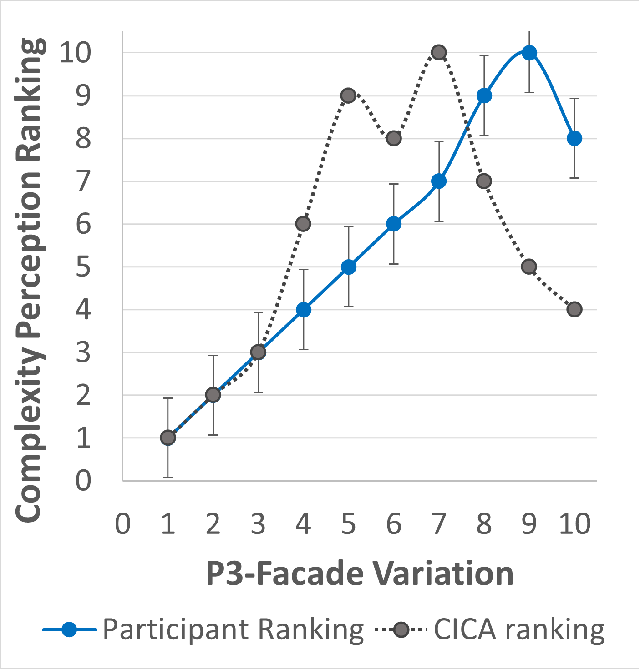
\includegraphics[width=\linewidth]{Images/AccuracyPattern3}
            \captionof{figure}{Accuracy comparison pattern 3 with original ranking}
            \label{fig:AccuracyPattern3}
        \end{tabularx}
    \end{table*}